%\documentclass{scrartcl}
%\usepackage{beamerarticle}
%%\usepackage{dtsc-beamer}
%\usepackage{fullpage}

\documentclass[9pt]{beamer}
\usetheme{boxes}
\usetheme{Boadilla}
\usecolortheme{beaver}
%\usecolortheme{sidebartab}
% \usefonttheme{structurebold}
\usefonttheme{serif}

%gets rid of bottom navigation bars
\setbeamertemplate{footline}[page number]{}

%gets rid of navigation symbols
\setbeamertemplate{navigation symbols}{}


% \usepackage{helvet}
\usepackage{amsmath, amssymb}
\usepackage{color}
%\usepackage{asymptote}
\usepackage{mathrsfs}
\usepackage{dsfont}
\usepackage{url}
\usepackage{cancel}
\usepackage{tikz}
\usetikzlibrary{fit,positioning}
\usetikzlibrary{shapes,matrix,decorations.markings,arrows}
\usetikzlibrary{graphs}
\usepackage{bbm}
\def\ind{\mathbbm{1}} %Indicator function
%
\definecolor{darkblue}{rgb}{0.0, 0.0, 0.55}
\definecolor{notsodarkblue}{rgb}{0.0, 0.0, 0.7}
\setbeamercolor{title}{fg=darkblue}
\setbeamercolor{frametitle}{fg=darkblue}
\newcommand{\myitem}{\item[$\bullet$]}
\definecolor{darkgreen}{rgb}{0, 0.55, 0}
\definecolor{lgray}{rgb}{0.9,0.9,0.9}

\newcommand{\LABFIG}[1]{\label{fig:#1}}%{\tt [fig:$\text{$#1$}$]}}



\newcommand{\ve}[1]{\boldsymbol{#1}}
\newcommand{\set}[1]{\mathcal{#1}}


\def\X{\ve{X}}
\def\x{\ve{x}}
\def\y{\ve{y}}
\def\Y{\ve{Y}}
\def\S{\ve{S}}
\def\s{\ve{s}}
\def\sg{\tilde{{s}}}
\def\n{n}
\def\C{\mathcal{C}}
\def\H{\ve{H}}
\newcommand{\st}[1]{{e}_{#1}}		%state
\newcommand{\str}[2]{{e}_{#2,(#1)}}	
\newcommand{\St}[1]{{E}_{#1}}		%state
\def\seqst{\ve{\st{}}}
\def\seqSt{\ve{\St{}}}
\def\S{\ve{S}}		%Symbol sequence
\def\AQAM{\mathcal{A}}
\def\Aest{\mathcal{E}}
\def\chl{\mathtt{h}} %Channel length
\def\s{\ve{s}} %transmitted word of symbols
\def\sk{{s}_k} %transmitted word of symbols 
\def\hsk{\hat{\s}_k}
\def\t{\mathtt{L}}   %Word length (symbols)

\def\eqtwo{\stackrel{\text{\tiny (mod 2)}}{=}}

\newcommand{\p}[1]{p_{_{#1}}} %pdf or pmf
\newcommand{\q}[1]{q_{_{#1}}} %pdf or pmf
\newcommand{\Iset}[1]{\mathtt{#1}} %Index set
\def\d{\text{d}}	%Differential (for integrals)

\newcommand{\mc}[1]{\mathcal{#1}}
\def\sX{\mc{X}}

\newcommand\Def[1]{{\textbf{Definition:}\\\emph{#1}\\\begin{center} ------------------------ \end{center}}}
\newcommand\Prop[1]{{\textbf{\textcolor{red}{Property:}}\\\emph{#1}\\\begin{center} \textcolor{red}{------------------------} \end{center}}}

\newcommand{\noteB}[1]{\textbf{\textcolor{notsodarkblue}{#1}}}

\newcommand{\noteR}[1]{\textbf{\textcolor{darkred}{#1}}}

\newcommand{\noteG}[1]{\textbf{\textcolor{darkgreen}{#1}}}

\newcommand{\snoteB}[1]{{\textcolor{darkblue}{#1}}}

\newcommand{\snoteR}[1]{{\textcolor{darkred}{#1}}}

\newcommand{\snoteG}[1]{{\textcolor{darkgreen}{#1}}}


\newcommand{\fs}[2]{#2}

\title[]{Introduction to Graphical Models and Inference for Communications}
\author[\textcolor{white}{Advanced Digital Communications}]{{\textcolor{black}{Pablo Martinez Olmos \\ olmos@tsc.uc3m.es}}
}
\date[]{{}}
\institute{\textcolor{white}{}}

% \pgfdeclareimage[height=0.5cm]{ITW}{pics/Logo.png}
%  \logo{\pgfuseimage{ITW}}

\AtBeginSection[]
{
  \begin{frame}<beamer>{Index}
    \tableofcontents[currentsection,currentsubsection]
  \end{frame}
}

\begin{document}

\frame{
\titlepage
\thispagestyle{empty}
\begin{center}
\includegraphics[scale=0.05]{Figuras/uc3m-logo.pdf}
\end{center}
}


\section{Course overview}

\frame{
\frametitle{\noteB{Graphical Models and approximate inference} 
}

\begin{itemize}
\item \snoteB{Exact inference over discrete trees: the Belief Propagation algorithm}.
%\item \snoteG{The forward/backward  algorithm is nothing but the BP algorithm}.
%\item \snoteR{BP for channel equalization.}
\item \snoteB{Approximate Inference over graphs with cycles using BP. }.
%\item \snoteG{Codes on graphs and iterative algorithms: achieve channel capacity at low-cost}.
%\item \snoteR{BP for binary and non-binary LDPC codes.}
\item \snoteB{Inference over Gaussian distributions using BP}.
%\item \snoteG{The Kalman Filter is nothing but the BP algorithm.}
%\item \snoteR{Gaussian message-passing on linear models. }
%\item \snoteG{Approximate message passing for Compressed Sensing.}
\item \snoteB{Beyond BP:  Mean field approximations, Expectation propagation and Monte Carlo approximations.}
%\item \snoteG{Approximate inference in digital-communication receivers.}
%\item \snoteR{Review of recent literature on the topic and expositions!}
\end{itemize}


}

\frame{
\frametitle{\noteB{Graphical Models and approximate inference} \noteG{ for  communications}
}

\begin{itemize}
\item \snoteB{Exact inference over discrete trees: the Belief Propagation algorithm}.
\begin{itemize}
\item \snoteG{The forward/backward BCJR  algorithm is nothing but the BP algorithm}.
\end{itemize}
%\item \snoteR{BP for channel equalization.}
\item \snoteB{Approximate Inference over graphs with cycles using BP. The Bethe approximation and beyond}.
\begin{itemize}
\item \snoteG{Codes on graphs and iterative algorithms: achieving channel capacity at low-cost}.
\end{itemize}
%\item \snoteR{BP for binary and non-binary LDPC codes.}
\item \snoteB{Inference over Gaussian distributions using BP}.
\begin{itemize}
\item \snoteG{The Kalman Filter is nothing but the BP algorithm.}
%\item \snoteG{Approximate message passing for Compressed Sensing.}
\end{itemize}
%\item \snoteR{Gaussian message-passing on linear models. }
\item \snoteB{Beyond BP:  Mean field approximations, Expectation propagation and Monte Carlo approximations.}
\begin{itemize}
\item \snoteG{Approximate inference in digital-communication receivers.}
\end{itemize}
%\item \snoteR{Review of recent literature on the topic and expositions!}
\end{itemize}


}

\frame{
\frametitle{\noteB{Graphical Models and approximate inference} \noteG{for  communications}
}

\noteR{Learning by programming and simulating algorithms ...}

\begin{itemize}
\item \snoteB{Exact inference over discrete trees: the Belief Propagation algorithm}.
\begin{itemize}
\item \snoteG{The forward/backward  algorithm is nothing but the BP algorithm}.
\item \snoteR{Bit-MAP decoding of convolutional codes using BP.}
\end{itemize}
\item \snoteB{Approximate Inference over graphs with cycles using BP. The Bethe approximation and beyond}.
\begin{itemize}
\item \snoteG{Codes on graphs and iterative algorithms: achieving channel capacity at low-cost}.
\item \snoteR{BP decoding of Turbo codes.}
\item \snoteR{BP decoding of binary  LDPC codes.}
\end{itemize}
\item \snoteB{Inference over Gaussian distributions using BP}.
\begin{itemize}
\item \snoteG{The Kalman Filter is nothing but the BP algorithm.}
\item \snoteG{Approximate message passing for Compressed Sensing.}
\item \snoteR{Gaussian message-passing on linear models.}
\end{itemize}
\item \snoteB{Beyond BP:  Mean field approximations, Expectation propagation and Monte Carlo approximations.}
\begin{itemize}
\item \snoteG{Approximate inference in digital-communication receivers.}
\item \snoteR{Iterative receivers for digital communications.}
\end{itemize}
\end{itemize}


}

%\frame{
%\frametitle{\noteB{Graphical Models and approximate inference} \noteG{for  communications}
%}
%
%\noteR{... and by reading papers together.}
%
%\begin{figure}
%\begin{tabular}{c}
%\includegraphics[scale=0.35]{Figuras/papers.pdf}
%\end{tabular}
%\end{figure}
%
%}


\frame{
\frametitle{Graphical Models}

\begin{itemize}
\item Graphical Models (GMs) bringht together graph theory and probability theory in a powerful formalism for multivariate statistical modeling.
\item \noteB{In a nutshell:} GMs use graphs to represent and manipulate joint probability distributions.
\end{itemize}

\begin{figure}
\begin{tabular}{c}
\includegraphics[scale=0.6]{Figuras/Graph_1.pdf}
\end{tabular}
\end{figure}

}


\frame{
\frametitle{You already know something about inference over GMs}

\begin{itemize}
\item Statistical models have long been formulated in terms of graphs in applied fields including bioinformatics, speech processing, image processing, coding theory in communications.
\end{itemize}

\begin{itemize}
\item Many widely known algorithms are expressed in terms of recursions operating on these graphs:
\begin{itemize}
\item Kalman filtering for state-space models.
\item Forward-backward algorithm for hidden Markov models.
\item Viterbi algorithm.
\item Iterative message passing decoders for LDPC codes.
\item ...
\end{itemize} 
\end{itemize}


\begin{block}{}
These ideas can be understood, unified and generalized within the formalism of graphical models.
\end{block}

}
%
%\frame{
%\frametitle{High-dimensional probability distributions}
%
%%\begin{itemize}
%%\item In fields that involve the study of large number of interacting variables, graphical models are increasing in evidence.
%%\end{itemize}
%\begin{itemize}
%\item Mathematically, the interactions in real-world systems are described by high-dimensional probability distributions.
%\end{itemize} 
%\begin{itemize}
%\item \noteR{High-dimensional probability distributions are  intractable} to learn and manipulate.
%\end{itemize}
%
%
%
%
%
%%
%
%
%
%
%
%}
%
%\frame{
%\frametitle{High-dimensional probability distributions}
%
%Consider a set of $d$ random binary variables $\X=(X_1,X_2,X_3,\ldots,X_n)$
%
%\begin{itemize}
%\item  \noteB{Storing} in a table all possible entries of the joint probability distribution $\p{\X}(\x)$ requires $2^{n}$ entries, unfeasible for $n\rightarrow\infty$.
%\item Even if we could store all values of $\p{\X}(\x)$, can we \noteB{learn} such distribution from samples? ($2^{n}$ probabilities to learn).
%\item Even if we could learn $\p{\X}(\x)$ and store it, can we make \noteB{inference}? Marginalizing cost $2^{n}$ binary sums!
%\end{itemize}
%
%\vspace{1cm}
%
%\noteR{Even on the most optimistically fast supercomputer this would take far too long,
%even for a $n = 100$ variable system.}
%
%}

\frame{
\frametitle{GMs to represent  probability distributions}

\begin{alertblock}{}
 Probabilistic graphical models are used to approximate such distributions by specifying a set of \noteB{conditional independence} or causality relationships, reducing the number of parameters needed to specify the distribution.
 \end{alertblock}

\vspace{1cm}

\begin{block}{}
Graph theory  also plays a fundamental role in assessing the \noteB{computational complexity of inference} algorithms over a GM.
\end{block}

\begin{figure}
\begin{tabular}{c}
\includegraphics[scale=0.6]{Figuras/Graph_1.pdf}
\end{tabular}
\end{figure}


}

\frame{
\frametitle{GMs: learn the model/learn from the model}


There are two main problems associated to graphical models:



\begin{enumerate}
\item Graphical Model Selection (Learn a graphical model from samples).
\item Efficient inference in Graphical Models.
\end{enumerate}


%FIRST PLOT: LEARNING GRAPHICAL MODEL STRUCTURE---> Given Data (set of channel outputs, noisy image or measurements, data from stock market) and a set of random variables that we estimate generated this data (transmitted symbols, pixels, traders) ---> Learn the graphical model! Everything could be connected to everything--> complexity reduction blah blah storage blah bla

%SECOND PLOT: INFERENCE. Given a graphical model --> we want to compute marginals or conditional probabilities. The structure of the graph is fundamental to asses the complexity/accuracity of inference methods. (General theme of shewoon slides)



}

\frame{
\frametitle{Graphical Model Selection}


\begin{figure}
\begin{tabular}{c}
\includegraphics[scale=0.35]{Figuras/Graph_3.pdf}
\end{tabular}
\end{figure}


}

\frame{
\frametitle{Exact Inference: the discrete case}

Let $\X$ be a discrete random vector and $\Y$ a noisy observation, where $\x\in\set{X}^n$, $\y\in\set{Y}^m$ and 
 the joint pmf is $\p{\X,\Y}(\x,\y)$. For a given observation $\Y=\y$, we are interested in drawing conclusions about $\X$. 

\vspace{0.5 cm}

Two basic kind of computations:

\begin{block}{}
Given $\Y=\y$, find the most probable realization of the posterior probability distribution: 
\begin{align*}
\hat{\x}&=\arg\max_{\x\in\set{X}^n} \p{\X|\y}(\x)=\arg\max_{\x\in\set{X}^n} \frac{\p{\Y|\x}(\y)\p{\X}(\x)}{\p{\Y}(\y)}=\arg\max_{\x\in\set{X}^n} \p{\Y|\x}(\y)\p{\X}(\x)
\end{align*}
\noteR{Complexity $\rightarrow$ $\mathcal{O}(|\set{X}|^n)$}.
\end{block}

}

\frame{
\frametitle{Exact Inference: the discrete case (II)}

\begin{block}{}
Given $\Y=\y$, compute the \emph{marginal} probability distribution $\p{X_i|\y}{(x_i)}$:
\begin{align*}
\p{X_i|\y}{(x_i)}&=\sum_{\x_{\sim i}\in\set{X}^{n-1}} \p{\X|\y}(\x)\\\nonumber
&=\frac{1}{\p{\Y}(\y)}\sum_{\x_{\sim i}\in\set{X}^{n-1}}\p{\Y|\x}(\y)\p{\X}(\x),
\end{align*}
\noteR{Complexity $\rightarrow$ $\mathcal{O}(|\set{X}|^n)$}.
\end{block}
}








%
%\frame{
%\frametitle{Inference over discrete probability distributions.}
%Given a probability distribution over $\X=(X_1,X_2,\ldots,X_d)$
%\begin{align*}
%\mu(\ve{x})=\mathbb{P}_{X_1,X_2,\ldots,X_d}(x_1,x_2,\ldots,x_d)
%\end{align*}
%where $x_i\in\sX$.
%\begin{itemize}
%\item Finding the most probable realization (mode):
%\begin{align*}
%\hat{\ve{x}}=\arg \max_{\ve{x}\in\sX^n}\mu(\ve{x})
%\end{align*}
%\item Compute marginals:
%\begin{align*}
%\mu(x_i)&=\sum_{\ve{x}\sim x_i}\mu(\ve{x})\qquad \text{Discrete case}\\
%\mu(x_i)&=\int_{\ve{x}\sim x_i}\mu(\ve{x})\qquad \text{Continuous case}
%\end{align*}
%\item Sampling (generate new samples from $\mu(\ve{x})$).
%\end{itemize}
%\begin{exampleblock}{}
%\centering Key challenge $n>>1$
%\end{exampleblock}
%}

\frame{
\frametitle{Structure helps!}
\begin{align*}
\p{\X}(\x)=\p{X_1}(x_1)\p{X_2|x_1}(x_2)\p{X_3|x_2}(x_3)\p{X_4|x_3}(x_4)\p{X_5|x_4}(x_5)
\end{align*}

\vspace{0.5cm}
How many operations we need to compute $\hat{\x}=\arg\max_{\x\in\set{X}^n}  \p{\X}(\x)$?

\begin{itemize}
\item \noteR{Brute force}: 5 variables $\Rightarrow |\set{X}|^5$ evaluations of $\p{\X}(\x)$
\item \noteB{Efficient Inference}: It is easy to check that it only costs $5 |\set{X}|^2$ function evaluations
\end{itemize}

\begin{exampleblock}{}
 When the probability distribution factorizes,
we can achieve huge computational gains. 
\end{exampleblock}

In other words...

\begin{block}{}
When the probability distribution is represented by a GM,
we can achieve huge computational gains. 
\end{block}



}

\frame{
\frametitle{Inference and GMs}

\begin{itemize}
\item  It is critical to understand for which graphical structures efficient inference (polynomial complexity with the dimension $n$) is possible.
\item We will use such knowledge to propose feasible and accurate \noteB{approximate inference methods} for those GMs for which  \noteB{exact inference} is prohibitively complex.
\end{itemize}



}


\frame{
\frametitle{Exact Inference: the continuous case}
Assume now that both $\X$ and $\Y$ are real-valued random vectors with joint pdf $\p{\X,\Y}(\x,\y)$ where $\x\in\set{\mathbb{R}}^n$ and $\y\in\set{\mathbb{R}}^m$ and that we observe $\Y=\y$.

\begin{block}{}
\begin{align*}
\hat{\x}=\arg\max_{\x\in\mathbb{R}^n} \p{\X|\y}(\x)=\arg\max_{\x\in\mathbb{R}^n} \frac{\p{\Y|\x}(\y)\p{\X}(\x)}{\p{\Y}(\y)}=\arg\max_{\x\in\mathbb{R}^n} \p{\Y|\x}(\y)\p{\X}(\x)\
\end{align*}
\noteR{Typically $ \p{\X|\y}(\x)$ is not convex and multimodal}
\end{block}

\begin{block}{}
\begin{align*}
\p{X_i|\y}{(x_i)} &=\int \p{\X|\y}(\x) \d\x_{\sim \Iset{i}}=\frac{1}{\p{\Y}(\y)}\int \p{\Y|\x}(\y)\p{\X}(\x) d\x_{\sim \Iset{i}}
\end{align*} 
\noteR{This integral lacks in general of analytical solution}
\end{block}

\noteB{Special case: Gaussian distribution}. 

}

\frame{
\frametitle{Structure helps!}

\begin{itemize}
\item Efficient \emph{approximate inferece} over $ \p{\X|\y}(\x)$ for real-valued distributions will be attained by constructing tractable approximation $\q{\X}(\x)$ where inference is possible.
\item Let $\q{\X}(\x|\ve{\theta})$ a family of distributions parameterized by a given vector $\ve{\theta}$. Assuming $\p{\X|\y}(\x)$ and $\q{\X}(\x|\ve{\theta})$ have the same support, two common criterions:
\begin{align*}
\q{\X}(\x|\hat{\ve{\theta}})&=\max_{\ve{\theta}} KL(\q{\X}||\p{\X})\qquad \text{Variational Inference}\\
\q{\X}(\x|\hat{\ve{\theta}})&=\max_{\ve{\theta}} KL(\p{\X}||\q{\X})\qquad \text{Expectation Propagation}
\end{align*}
\item Feasible methods exploit the properties of the GM that represents $\p{\X|\y}(\x)$! 
\end{itemize}
}


\section{Representing probability distributions via Factor graphs}

\frame{
\frametitle{Graphical models}
\begin{itemize}
\item There are three main graph-based languages for describing probability distributions: \noteG{Bayessian Networks} (directed graphs), \noteB{Markov Random Fields} (undirected graphs) and \noteB{Factor graphs}.
\end{itemize}
\begin{itemize}
\item  They differ in the set of conditional independences they can encode and in the factorization of the distribution that they induce.
\end{itemize}
\begin{itemize}
\item  For the purpose of solving inference problems, \noteB{it is often convenient to convert both directed and undirected graphs into factor graphs}.
\end{itemize}




}






\subsection{Directed graphical models}

\frame{
\frametitle{Bayesian networks (directed graphical models)}
\begin{itemize}
\item They efficiently represent large joint distributions by making a set of \noteB{conditional independence} (CI) assumptions.
\begin{align*}
X\perp Y| Z \Leftrightarrow \p{X,Y|z}(x,y)=\p{X|z}(x)\p{Y|z}(y)
\end{align*}
\end{itemize}



\begin{itemize}
\item A Bayesian network is a probability distribution of the form
\begin{align*}
\p{\X}(\x)=\prod_{i=1}^{n}\p{X_i|\ve{x}^{\pi}_i}(x_i)
\end{align*}
where $\ve{x}^{\pi}_i$ is the set of parents of $X_i$.
\item Represented as a \textbf{directed graph}.
\end{itemize}

\begin{figure}
\includegraphics[scale=0.5]{Figuras/Graph_4.pdf}  
\end{figure}
$\p{\X}(\x)=\p{X_1}(x_1)\p{X_2}(x_2)\p{X_3|x_1,x_2}(x_3)\p{X_5}(x_5)\p{X_4|x_3,x_5}(x_4)\p{X_6|x_1}(x_6)$




}
%
%\frame{
%\begin{itemize}
%\item BNs are well-suited to use known causal relationships and to express conditional dependences between variables in the graph.
%\end{itemize}
%
%\begin{block}{Medical diagnosis with the t quick medical reference (QMR) network}
%Both diseases $\ve{D}$ and symptoms $\ve{S}$ are binary random variables. The conditional probabilities  are represented by the \emph{noisy-OR model}:%\footnote{Pmf for discrete variables are denoted by $P(x)$}:
%\begin{align*}
%\p{S_j|\ve{d}}(s_j=0)=(1-\theta_{0,i})\prod_{i\in\pi_{s_j}}(1-\theta_{i,j})^{d_j}
%\end{align*}
%\end{block}
%
%
%\begin{figure}
%\begin{tabular}{c}
%\includegraphics[scale=0.2]{Figuras/Graph_6.pdf}
%\end{tabular}
%\end{figure}
%
%\begin{alertblock}{}
%Given real data, we try to learn the $\theta_{i,j}$ parameters.
%\end{alertblock}
%
%}
%
%\frame{
%\frametitle{Inference over the QMR network}
%\begin{itemize}
%\item If we observe a certain set $\mc{S}$ of symptoms, what is the probability that the patient suffers from disease $d_j$?
%\begin{align*}
%P(s_j,|\ve{d}_{\mc{S}})=\sum_{\ve{s}\sim s_j}\sum_{\ve{d}\sim \ve{d}_{\mc{S}}} P(\ve{s},\ve{d})
%\end{align*}
%\end{itemize}
%
%\begin{figure}
%\begin{tabular}{c}
%\includegraphics[scale=0.2]{Figuras/Graph_7.pdf}
%\end{tabular}
%\end{figure}
%
%\begin{block}{}
%\begin{itemize}
%\item Exact calculation needs $2^{569+4075-|S|}$ sums!!
%\item We will study methods for approximate inference.
%\end{itemize}
%\end{block}
%
%}
%
%\frame{
%\frametitle{Evaluating CI is hard in BNs}
%
%Given a BN
%\begin{align*}
%\mu(\ve{x})=\prod_{i=1}^{d}\mu(x_i|\ve{x}_{\pi(x_i)})
%\end{align*}
%if we consider a partition of the variable in the directed graph into three sets $A$, $B$ and $C$, evaluating whether
%\begin{align*}
%\X_A\perp \X_B| \ve{x}_E 
%\end{align*}
%is not trivial (see $d$-separation theorem and the Bayes Ball algorithm).
%
%\begin{block}{Why are we interested in CI?}
%Structure helps to efficiently solve inference problems!
%\end{block}
%
%}
%
%\frame{
%\begin{figure}
%\begin{tabular}{c}
%\includegraphics[scale=0.2]{Figuras/Graph_8.pdf}
%\end{tabular}
%\end{figure}
%
%\begin{exampleblock}{With no CI assumptions (no BNs)}
%$|\sX|^{|A|+|B|+|C|}$ sums!
%\end{exampleblock}
%
%
%}
%
%
%\frame{
%
%\begin{block}{If we exploit $\X_B\perp\X_C|\X_A$}
%\begin{align*}
%P(x_j)&=\sum_{\ve{x}_{A}}\sum_{\ve{x}_{B}}\sum_{\ve{x}_{C}\sim x_{j}}P(\ve{x}_{A})P(\ve{x}_{B}|\ve{x}_{A})P(\ve{x}_{C}|\ve{x}_{A})\\
%&=\sum_{\ve{x}_{A}}P(\ve{x}_{A}) \underbrace{\left(\sum_{\ve{x}_{B}} P(\ve{x}_{B}|\ve{x}_{A}) \right)}_{=1 ~ \forall \ve{x}_{A}}\left(\sum_{\ve{x}_{C}\sim x_{j}} P(\ve{x}_{C}|\ve{x}_{A}) \right)
%\end{align*}
%The  cost to compute the marginal by brute-force is reduced to $|\sX|^{|A|+|B|}$.
%\end{block}
%
%
%}
%
%\frame{
%
%\Def{ the Markov Blanket of a given set of random variables $\X_S$ is the set of variables $\X_{M(S)}$ such that
%\begin{align*}
%\X_S \perp \X_{\text{rest of the graph}}|\X_{M(S)}
%\end{align*}
%}
%
%Evaluating the Markov Blanket is BNs is not intuitive.
%
%}


\frame{
\frametitle{Hidden Markov Models}

\begin{itemize}
\item BNs are well-suited to use known causal relationships and to express conditional dependences between variables in the graph.
\end{itemize}

\begin{itemize}
\item HMMs are naturally represented by BNs.
\end{itemize}

\begin{figure}
\begin{tabular}{c}
\includegraphics[scale=0.5]{Figuras/Graph_17_2.pdf}
\end{tabular}
\end{figure}

\begin{align*}
\p{\X,\Y}(\x,\y)&=\p{\X_1}(\x_1)\p{\Y_1|\x_1}(\y_1)\p{\X_2|\x_1}(\x_2)\p{\Y_2|\x_2}(\y_2)\ldots\p{\X_t|\x_{t-1}}(\x_t)\p{\Y_t|\x_t}(\y_t)
\end{align*}



}

\subsection{Undirected graphical models}


\frame{
\frametitle{Markov Random Fields (MRFs)}
\begin{itemize}
\item Also called undirected graphical models.
\item For some domains, being force to choose a direction for the edges, as required by BNs, is unnatural.
\item MRFs do not require to specify orientations. 
\item They are more natural for domains such as spatial or relational data. Widely used in image analysis and spatial statistics. 
\item Less interpretable as BNs.
\item \noteB{More flexible}. Factors are \noteG{arbitrary positive functions} (potentials).
\end{itemize}



}

\frame{

For a random vector $\x$, a MRF is defined as follows
\begin{align*}
\p{\X}(\x)=\frac{1}{Z}\prod_{c=1}^{C}\phi_{c}(\x_c),
\end{align*}
where 
\begin{enumerate}
\item $\X_c$ $c=1,\ldots,C$ are non-disjoint groups of variables.
\item All groups are maximal (there is no $(c,d)$ such that $\X_c\subseteq\X_d$).
\item $\phi_{c}(\x_c): \sX^{|C|}\rightarrow \mathbb{R}^{+}$ (a.k.a. potential functions)
\item $Z$ is a normalization constant:
\begin{align*}
Z&=\int_{\sX^n} \prod_{c=1}^{C}\phi_{c}(\x_c) \text{d}\x, \qquad Z=\sum_{\sX^n} \prod_{c=1}^{C}\phi_{c}(\x_c) 
\end{align*}
\end{enumerate}



}

\frame{
\begin{itemize}
\item Graphically, we represent a MRF by an undirected graph where all variables in $\X_c$ are connected to each other (clique).
\end{itemize}

\begin{figure}
\begin{tabular}{c}
\includegraphics[scale=0.5]{Figuras/Graph_9.pdf}
\end{tabular}
\end{figure}


}
%
%\frame{
%\begin{itemize}
%\item Cliques correspond to maximal groups (maximal cliques).
%\item There is no clique (fully connected subgraph) contained in another clique.
%\end{itemize}
%
%\begin{figure}
%\begin{tabular}{c}
%\includegraphics[scale=0.7]{Figuras/Graph_10.pdf}
%\end{tabular}
%\end{figure}
%
%}
%
%\frame{
%
%\begin{figure}
%\begin{tabular}{c}
%\includegraphics[scale=0.45]{Figuras/Graph_11.pdf}
%\end{tabular}
%\end{figure}
%
%
%
%}
%
\frame{
\frametitle{Evaluating conditional independence in MRF}
\Prop{In a MRF, if a group of conditioned (observed) variables $\X_o$ is such that all paths from $\X_A$ to $\X_B$ go through $\X_o$, then 
\begin{align*}
\X_A\perp \X_B| \X_o
\end{align*}
  }
  
  \begin{figure}
\begin{tabular}{c}
\includegraphics[scale=0.45]{Figuras/Graph_12.pdf}
\end{tabular}
\end{figure}



}


\frame{
\frametitle{Markov Blanket in MRFs}


  \begin{figure}
\begin{tabular}{c}
\includegraphics[scale=0.45]{Figuras/Graph_13.pdf}
\end{tabular}
\end{figure}



}

\frame{
\frametitle{Markov Blanket in MRFs}


  \begin{figure}
\begin{tabular}{c}
\includegraphics[scale=0.45]{Figuras/Graph_14.pdf}
\end{tabular}
\end{figure}



}

%\frame{
%\frametitle{From BNs to MRFs}
%\begin{itemize}
%\item Converting BNs into MRFs graphs is relatively easy.
%\item However, it typically results into more dense graphs.
%\item Complexity/performance of basic inference methods is related with the sparseness of the graph.
%\item \noteR{Conversion might not be a good idea}.
%\item \noteG{There are some algorithms that are only defined for MRFs}.
%\end{itemize}
%
%}

%
%\frame{
%
%\begin{block}{}
%What is the Markov Blanket of $X_3$?
%\end{block}
%
%  \begin{figure}
%\begin{tabular}{c}
%\includegraphics[scale=0.6]{Figuras/Graph_15_2.pdf}
%\end{tabular}
%\end{figure}
%
%$$\p{\X}(\x)=\p{X_1}(x_1)\p{X_2}(x_2)\p{X_3|x_1,x_2,x_5}(x_3)\p{X_5}(x_5)\p{X_4|x_3,x_5,x_6}(x_4)\p{X_6|x_1}(x_6)$$
%
%}
%
%\frame{
%
%
%  \begin{figure}
%\begin{tabular}{c}
%\includegraphics[scale=0.6]{Figuras/Graph_16_2.pdf}
%\end{tabular}
%\end{figure}
%
%$$\p{\X}(\x)=\color{darkblue}{\overbrace{\p{X_1}(x_1)\p{X_2}(x_2)\p{X_3|x_1,x_2,x_5}(x_3)}^{{\phi_1(\x_1)}}}\color{darkred}{\underbrace{\p{X_5}(x_5)\p{X_4|x_3,x_5,x_6}(x_4)}_{\phi_2(\x_2)}}\color{darkgreen}{\overbrace{\p{X_6|x_1}(x_6)}^{\phi_3(\x_3)}}$$
%
%\begin{exampleblock}{}
%The graph is denser :( ... but we can easily determine the Markov Blanket of $X_3$ :).
%\end{exampleblock}
%
%}
%
%\frame{
%\frametitle{Image Modeling using MRFs}
%
%  \begin{figure}
%\begin{tabular}{c}
%\includegraphics[scale=0.6]{Figuras/Graph_19.pdf}
%\end{tabular}
%\end{figure}
%
%}
%
%\frame{
%\frametitle{Image Modeling using MRFs}
%
%  \begin{figure}
%\begin{tabular}{c}
%\includegraphics[scale=0.6]{Figuras/Graph_20.pdf}
%\end{tabular}
%\end{figure}
%
%}

\subsection{Factor graphs}

\frame{
\frametitle{Factor Graphs}

\begin{itemize}
\item As  MRFs, they are convenient to model soft constraints between random variables that are not naturally given as a conditional probability.
\item  Factor graphs (FGs) make the factorization of a distribution explicit in the graph by introducing additional nodes for the factor themselves.
\item They can preserve more details about the factorization.
\item For the purpose of solving \noteB{inference} problems, it is often \noteR{convenient to convert both directed and undirected graphs into factor graphs.}
\end{itemize}

\begin{exampleblock}{}
In many probabilistic models in communications, the joint distribution is expressed as large product of functions that overlap in their dependencies. In these scenarios, FGs are highly recommended since an equivalent MRF would produce an almost fully connected graph. 
\end{exampleblock}


}

\frame{
\frametitle{Factor Graphs (FGs)}
\Def{Given a probability distribution
\begin{align*}
\p{\X}(\x)=\frac{1}{Z}\prod_{j\in\Iset{J}}t_j(\x_{j})
\end{align*}
The FG has a node (represented by a square) for each factor $t_j$, $j\in\Iset{J}$ and a variable node (represented by a circle) for each variable $x_i$, $i=1,\ldots,n$.  For each $x_i\in\x_j$, we place an undirected link between factor $t_j$ and variable $x_i$.
}

\begin{block}{}
FGs simply describe the factorization of functions.
\end{block}

\begin{block}{}
They are bipartite graphs.
\end{block}





}

\frame{

\begin{align*}
\p{\X}(\x)=\frac{1}{Z} t_1(x_1,x_2) t_2(x_2,x_3,x_4) t_3(x_3,x_5)t_4(x_4)t_5(x_4,x_5), \qquad \x\in\set{X}^5
\end{align*}

\begin{center}
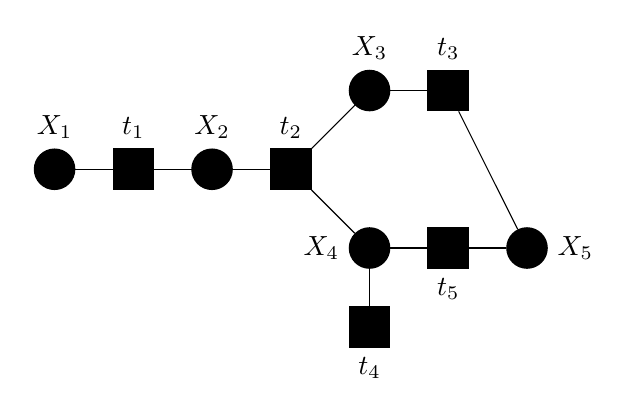
\begin{tikzpicture}[scale=1]
\tikzstyle{factor}=[rectangle,minimum size = 5mm, thick, draw =black,fill=black]
\tikzstyle{var}=[circle,minimum size = 5mm, thick, draw =black,fill=black]
\tikzstyle{second}=[circle, minimum size = 10mm, thick]
\tikzstyle{box}=[rectangle, draw=black!100]
\tikzstyle{connect}=[-latex, thick]
\draw[step=5cm];
	\node[var] (x_1) at (-1,0) [label=above:{$X_1$}]{};
	\node[factor] (t_1) at (0,0) [label=above:{$t_1$}]{};
	\node[var] (x_2) at (1,0) [label=above:{$X_2$}]{};
	\node[factor] (t_2) at (2,0) [label=above:{$t_2$}]{};
	\node[var] (x_3) at (3,1) [label=above:{$X_3$}]{};
	\node[factor] (t_3) at (4,1) [label=above:{$t_3$}]{};
	\node[var] (x_4) at (3,-1) [label=left:{$X_4$}]{};
	\node[factor] (t_4) at (3,-2) [label=below:{$t_4$}]{};
	\node[factor] (t_5) at (4,-1) [label=below:{$t_5$}]{};
	\node[var] (x_5) at (5,-1) [label=right:{$X_5$}]{};
	
	
	\path
		(x_1) edge []  (t_2) 
		(t_2) edge [] (x_3) 
		(x_3) edge [] (t_3)
		(t_2) edge [] (x_4)
		(t_4) edge [] (x_4)
		(x_4) edge [] (x_5)
		(t_3) edge [] (x_5);
		
\end{tikzpicture}
\end{center}



}

\frame{

By defining $\S=[\begin{array}{ccc} X_3 & X_4 & X_5 \end{array}]^T$, the same distribution factorizes as follows 

\begin{align*}
\p{\X}(\x)&=\frac{1}{Z} t_1(x_1,x_2) t_2(x_2,x_3,x_4) t_3(x_3,x_5)t_4(x_4)t_5(x_4,x_5)\\\\
\p{\X}(\x)&=\frac{1}{Z} t_1(x_1,x_2) t_2(x_2,\s) t_s(\s), 
\end{align*}

\begin{center}
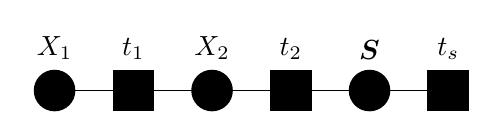
\begin{tikzpicture}[scale=1]
\tikzstyle{factor}=[rectangle,minimum size = 5mm, thick, draw =black,fill=black]
\tikzstyle{var}=[circle,minimum size = 5mm, thick, draw =black,fill=black]
\tikzstyle{second}=[circle, minimum size = 10mm, thick]
\tikzstyle{box}=[rectangle, draw=black!100]
\tikzstyle{connect}=[-latex, thick]
\draw[step=5cm];
	\node[var] (x_1) at (-1,0) [label=above:{$X_1$}]{};
	\node[factor] (t_1) at (0,0) [label=above:{$t_1$}]{};
	\node[var] (x_2) at (1,0) [label=above:{$X_2$}]{};
	\node[factor] (t_2) at (2,0) [label=above:{$t_2$}]{};
	\node[var] (s) at (3,0) [label=above:{$\S$}]{};
	\node[factor] (t_s) at (4,0) [label=above:{$t_s$}]{};
	
	
	\path
		(x_1) edge []  (t_2) 
		(t_2) edge [] (s) 
		 (s) edge [] (t_s);
		
\end{tikzpicture}
\end{center}

\begin{block}{}
Factors can be merged/split arbitrarily, allowing further algorithmic development for efficient inference.
\end{block}

\begin{alertblock}{Clustering of variable/factor nodes}
It does not changes the global probability distribution but defines a new graph where, at the expense of more complex potential functions and losing representation of conditional independency constraints,  approximate inference methods provide more accurate estimates.
\end{alertblock}

}


%
%\frame{
%However, assessing CI can be difficult in FGs 
%\begin{figure}
%\begin{tabular}{c}
%\includegraphics[scale=0.6]{Figuras/Graph_24.pdf}
%\end{tabular}
%\end{figure}
%
%
%}

%\frame{
%\frametitle{Summarizing...}
%
%\begin{itemize}
%\item For most the  applications in communications of efficient inference over GMs, we will use FGs.
%\item In other fields, BNs and MRFs are widely used.
%\item Algorithms may require specific GMs representations.
%\item In any case, recall that the graph properties (density, cycles, minimum distance paths etc...) and CI between regions of the graph are extremely linked with how efficient can inference be made. 
%\end{itemize}
%
%
%}

%\section{Examples in Communications}

%\frame{

%}

\section{Factor graphs in digital communications scenarios}

\subsection{Transmission of linear block codes over a memoryless channel}
\frame{
\frametitle{Transmission of linear block codes over a memoryless channel}
\begin{itemize}
\item A binary codeword $\x=(x_1,x_2,\ldots,x_\n)$ is randomly selected from a linear block code $\C$ of length $\n$.
\item Assume a Hamming (7,4) linear block code with $\n=7$ and parity check matrix:
\begin{align*}
\H=\left[ \begin{array}{ccccccc} 1 & 0 & 1 & 0 & 1 & 0 & 1\\ 0 & 1 & 1 & 0 & 0 & 1 & 1\\ 0 & 0 & 0 & 1 & 1 & 1 & 1\end{array}\right],
\end{align*}
\item Hence, every codeword $\x=(x_1,x_2,\ldots,x_7)$ have to fulfill the following parity-check equations:
\begin{align*}
x_1\oplus x_3\oplus x_5\oplus x_7=0\\
x_2\oplus x_3\oplus x_6\oplus x_7=0\\
x_4\oplus x_5\oplus x_6\oplus x_7=0
\end{align*}
\end{itemize}
}

\frame{
\begin{itemize}
\item  $\x\in\C$ is transmitted over a memoryless channel so that every output $y_i$ depends just on $x_i$.
\item For a given channel observation $\y$, the joint posterior probability of the transmitted codeword is expressed as 
\begin{align*}
\p{\X|\y}(\x)=\frac{\p{\Y|\x}(\y)\;\p{\X}(\x)}{\p{\Y}(\y)}\propto\p{\X}(\x)\prod_{i=1}^{n}\p{Y_i|x_i}(y_i),
\end{align*}
where
\begin{align*}
\p{\X}(\x)=\frac{\ind[\x\H^T\eqtwo\ve{0}]}{|\C|}.
\end{align*}
\item This last term can be further factorized. Let  $\ve{d}(\x)\doteq\x\H$ (mod 2) be the \emph{syndrome} vector, of length $n-k$ (number of rows of $\H$)
\begin{align*}
\p{\X}(\x)=\frac{\displaystyle\prod_{j=1}^{n-k}\ind[d_j(\x)\eqtwo0]}{|\C|}
\end{align*}
\end{itemize}

}

\frame{
Finally ...
\begin{align*}
\p{\X|\y}(\x)=\frac{1}{|\C|\p{\Y}(\y)}\prod_{j=1}^{n-k}\ind\left[d_j(\x)\eqtwo0 \right] \prod_{i=1}^{\n}\p{Y_i|x_i}(y_i).
\end{align*}

\begin{figure}[h] 
\centering\includegraphics[scale=0.6]{Figuras/Fig1_3.pdf}
 \end{figure}

}

\frame{
\begin{block}{Block-wise maximum a posteriori decoder (block-MAP decoding)}
\begin{align*}
\hat{\x}=\arg\max_{\x\in\C}\p{\X|\y}(\x)=\arg\max_{\x\in\C}\prod_{j=1}^{n-k}\ind[d_j(\x)\eqtwo0]\prod_{i=1}^{n}\p{Y_i|x_i}(y_i),
\end{align*}
\end{block}
\begin{exampleblock}{Symbol-wise maximum a posteriori decoder (symbol-MAP)}
\begin{align*}
\hat{x}_i&=\arg\max_{x_i\in\{0,1\}}\p{X_i|\y}(x_i)=\arg\max_{x_i\in\{0,1\}} \sum_{\x_{\sim i}\in\{0,1\}^{n-1}}\p{\X|\y}(\x)\\
&=\arg\max_{x_i\in\{0,1\}} \sum_{\x_{\sim i}\in\{0,1\}^{n-1}} \prod_{j=1}^{n-k}\ind[d_j(\x)\eqtwo0]\prod_{i=1}^{n}\p{Y_i|x_i}(y_i) 
\end{align*}
\end{exampleblock}
\begin{itemize}
\item \noteR{Both have $\mathcal{O}(2^n)$ complexity.}
\end{itemize}
}

\subsection{Symbol transmission and detection over ISI channels}
\frame{
\frametitle{Symbol transmission and detection over ISI channels}
\begin{itemize}
\item Consider a sequence of $\t$ i.i.d. $M$-ary  complex-valued  symbols, $\sk$, obtained by the encoding of a sequence of information bits. 
\item $s_k\in\AQAM$ and $|\AQAM|=M$.
\item  ISI channel that also introduces additive white Gaussian noise (AWGN):
\begin{align*}
y_k=\sum_{i=0}^{\chl}h_{i}s_{k-i}+w_k, \qquad w_k\sim\mathcal{CN}(\ve{0},\sigma_w^2\mathbf{I})
\end{align*}
\item The sequence of symbols $\s$ is preceded and terminated by a sequence of $\chl$ deterministic known symbols: $s_k=s^*$ for $k\in\{-\chl+1,\ldots,0\}$ and for $k\in\{\t+1,\ldots,\sk+\chl\}$.
\item $\y=(y_1,y_2,\ldots,y_{\t+\chl})$ is the observation vector.
\end{itemize}

%
%\begin{center}
%\begin{tikzpicture}[scale=1]
%\tikzstyle{factor}=[rectangle,minimum size = 5mm, thick, draw =black,fill=black]
%\tikzstyle{var}=[circle,minimum size = 5mm, thick, draw =black,fill=black]
%\tikzstyle{second}=[circle, minimum size = 10mm, thick]
%\tikzstyle{box}=[rectangle, draw=black!100]
%\tikzstyle{connect}=[-latex, thick]
%\draw[step=5cm];
%	\node[var] (x_1) at (-1,0) [label=above:{$X_1$}]{};
%	\node[factor] (t_1) at (0,0) [label=above:{$t_1$}]{};
%	\node[var] (x_2) at (1,0) [label=above:{$X_2$}]{};
%	\node[factor] (t_2) at (2,0) [label=above:{$t_2$}]{};
%	\node[var] (x_3) at (3,1) [label=above:{$X_3$}]{};
%	\node[factor] (t_3) at (4,1) [label=above:{$t_3$}]{};
%	\node[var] (x_4) at (3,-1) [label=left:{$X_4$}]{};
%	\node[factor] (t_4) at (3,-2) [label=below:{$t_4$}]{};
%	\node[factor] (t_5) at (4,-1) [label=below:{$t_5$}]{};
%	\node[var] (x_5) at (5,-1) [label=right:{$X_5$}]{};
%	
%	
%	\path
%		(x_1) edge []  (t_2) 
%		(t_2) edge [] (x_3) 
%		(x_3) edge [] (t_3)
%		(t_2) edge [] (x_4)
%		(t_4) edge [] (x_4)
%		(x_4) edge [] (x_5)
%		(t_3) edge [] (x_5);
%		
%\end{tikzpicture}
%\end{center}



}

\frame{
\begin{align*}
\p{\S|\y}(\s)=\frac{\color{darkred}{}\p{\Y|\s}(\y)\color{black}\p{\S}(\s)}{\p{\Y}(\y)}%\propto \prod_{k=1}^{\t+\chl}\p{Y_k|\{s_j\}_{j=k-\chl}^{k}}(y_k) \p{S_k}(s_k)
% \cdot \prod_{k=t+1}^{\t+\chl}\p{Y_k|\{S_j=s_j\}_{j=k-\chl}^{t}}(y_k) 
\end{align*}
%where 
%\begin{itemize}
%\item $\p{S_k}(s_k)=1/M$ for $s_k\in\AQAM$ for $k=1,\ldots,s$.
%\item $\p{S_k}(s_k)=\ind[S_k=s^*]$ for $k=\t+1,\ldots,\t+\chl$.
%\end{itemize}
}

\frame{
\begin{align*}
&\p{\S|\y}(\s)=\frac{\color{darkred}{}\p{\Y|\s}(\y)\color{black}\p{\S}(\s)}{\p{\Y}(\y)}\\\\%\propto \prod_{k=1}^{\t+\chl}\p{Y_k|\{s_j\}_{j=k-\chl}^{k}}(y_k) \p{S_k}(s_k)
% \cdot \prod_{k=t+1}^{\t+\chl}\p{Y_k|\{S_j=s_j\}_{j=k-\chl}^{t}}(y_k) 
&\p{\Y|\s}(\y)=\prod_{k=1}^{\t+\chl}\p{Y_k|\s}(y_k)%=\prod_{k=1}^{\t+\chl}\p{Y_k|\{s_j\}_{j=k-\chl}^{k}}(y_k)
\end{align*}
%where 
%\begin{itemize}
%\item $\p{S_k}(s_k)=1/M$ for $s_k\in\AQAM$ for $k=1,\ldots,s$.
%\item $\p{S_k}(s_k)=\ind[S_k=s^*]$ for $k=\t+1,\ldots,\t+\chl$.
%\end{itemize}
}

\frame{
\begin{align*}
&\p{\S|\y}(\s)=\frac{\color{darkred}{}\p{\Y|\s}(\y)\color{black}\p{\S}(\s)}{\p{\Y}(\y)}\\\\%\propto \prod_{k=1}^{\t+\chl}\p{Y_k|\{s_j\}_{j=k-\chl}^{k}}(y_k) \p{S_k}(s_k)
% \cdot \prod_{k=t+1}^{\t+\chl}\p{Y_k|\{S_j=s_j\}_{j=k-\chl}^{t}}(y_k) 
&\p{\Y|\s}(\y)=\prod_{k=1}^{\t+\chl}\p{Y_k|\s}(y_k)=\color{darkred}{}\prod_{k=1}^{\t+\chl}\p{Y_k|\{s_j\}_{k-\chl}^{k}}(y_k)
\end{align*}
%where 
%\begin{itemize}
%\item $\p{S_k}(s_k)=1/M$ for $s_k\in\AQAM$ for $k=1,\ldots,s$.
%\item $\p{S_k}(s_k)=\ind[S_k=s^*]$ for $k=\t+1,\ldots,\t+\chl$.
%\end{itemize}
}


\frame{
\begin{align*}
&\p{\S|\y}(\s)=\frac{\color{darkred}{}\p{\Y|\s}(\y)\color{darkgreen}\p{\S}(\s)}{\p{\Y}(\y)}\\\\%\propto \prod_{k=1}^{\t+\chl}\p{Y_k|\{s_j\}_{j=k-\chl}^{k}}(y_k) \p{S_k}(s_k)
% \cdot \prod_{k=t+1}^{\t+\chl}\p{Y_k|\{S_j=s_j\}_{j=k-\chl}^{t}}(y_k) 
&\p{\Y|\s}(\y)=\prod_{k=1}^{\t+\chl}\p{Y_k|\s}(y_k)=\color{darkred}{}\prod_{k=1}^{\t+\chl}\p{Y_k|\{s_j\}_{k-\chl}^{k}}(y_k)\\\\
&\color{darkgreen}\p{\S}(\s)=\prod_{u=-\chl+1}^{\t+\chl}\p{S_u}(s_u)
%\\\\&\color{darkgreen}{}\p{S_u}(s_u)=1/M \text{ for } s_u\in\AQAM \text{ and } u=1,\ldots,s\\\\
\end{align*}
}

\frame{
\begin{align*}
&\p{\S|\y}(\s)=\frac{\color{darkred}{}\p{\Y|\s}(\y)\color{darkgreen}\p{\S}(\s)}{\p{\Y}(\y)}\\\\%\propto \prod_{k=1}^{\t+\chl}\p{Y_k|\{s_j\}_{j=k-\chl}^{k}}(y_k) \p{S_k}(s_k)
% \cdot \prod_{k=t+1}^{\t+\chl}\p{Y_k|\{S_j=s_j\}_{j=k-\chl}^{t}}(y_k) 
&\p{\Y|\s}(\y)=\prod_{k=1}^{\t+\chl}\p{Y_k|\s}(y_k)=\color{darkred}{}\prod_{k=1}^{\t+\chl}\p{Y_k|\{s_j\}_{k-\chl}^{k}}(y_k)\\\\
&\color{darkgreen}\p{\S}(\s)=\prod_{u=-\chl+1}^{\t+\chl}\p{S_u}(s_u)
\\\\&\color{darkgreen}{}\p{S_u}(s_u)=1/M \text{ for } s_u\in\AQAM \text{ and } u=1,\ldots,s\\\\
\end{align*}
}

\frame{
\begin{align*}
&\p{\S|\y}(\s)=\frac{\color{darkred}{}\p{\Y|\s}(\y)\color{darkgreen}\p{\S}(\s)}{\p{\Y}(\y)}\\\\%\propto \prod_{k=1}^{\t+\chl}\p{Y_k|\{s_j\}_{j=k-\chl}^{k}}(y_k) \p{S_k}(s_k)
% \cdot \prod_{k=t+1}^{\t+\chl}\p{Y_k|\{S_j=s_j\}_{j=k-\chl}^{t}}(y_k) 
&\p{\Y|\s}(\y)=\prod_{k=1}^{\t+\chl}\p{Y_k|\s}(y_k)=\color{darkred}{}\prod_{k=1}^{\t+\chl}\p{Y_k|\{s_j\}_{k-\chl}^{k}}(y_k)\\\\
&\color{darkgreen}\p{\S}(\s)=\prod_{u=-\chl+1}^{\t+\chl}\p{S_u}(s_u)
\\\\&\color{darkgreen}{}\p{S_u}(s_u)=1/M \text{ for } s_u\in\AQAM \text{ and } u=1,\ldots,\t\\\\
&\color{darkgreen}{}\p{S_u}(s_u)= \ind[s_u=s^*] \text{ for }  u\in\{-\chl+1,\ldots,0\} \text{ and } u\in\{\t+1,\ldots,\chl+\chl\}
\end{align*}
}


%\frame{
%\begin{align*}
%\p{\S|\y}(\s)=\frac{\p{\Y|\s}(\y)\p{\S}(\s)}{\p{\Y}(\y)}\propto \prod_{k=1}^{\t+\chl}\p{Y_k|\{s_j\}_{j=k-\chl}^{k}}(y_k) \p{S_k}(s_k)
%% \cdot \prod_{k=t+1}^{\t+\chl}\p{Y_k|\{S_j=s_j\}_{j=k-\chl}^{t}}(y_k) 
%\end{align*}
%where 
%\begin{itemize}
%\item $\p{S_k}(s_k)=1/M$ for $s_k\in\AQAM$ for $k=1,\ldots,s$.
%\item $\p{S_k}(s_k)=\ind[S_k=s^*]$ for $k=\t+1,\ldots,\t+\chl$.
%\end{itemize}
%
%
%}

\frame{

\begin{align*}
\p{\S|\y}(\s)=\frac{\p{\Y|\s}(\y)\p{\S}(\s)}{\p{\Y}(\y)}\propto \prod_{k=1}^{\t+\chl}\p{Y_k|\{s_j\}_{k-\chl}^{k}}(y_k) \prod_{u=-\chl+1}^{\t+\chl}\p{S_u}(s_u) 
% \cdot \prod_{k=t+1}^{\t+\chl}\p{Y_k|\{S_j=s_j\}_{j=k-\chl}^{t}}(y_k) 
\end{align*}


\begin{figure}[h]
\centering
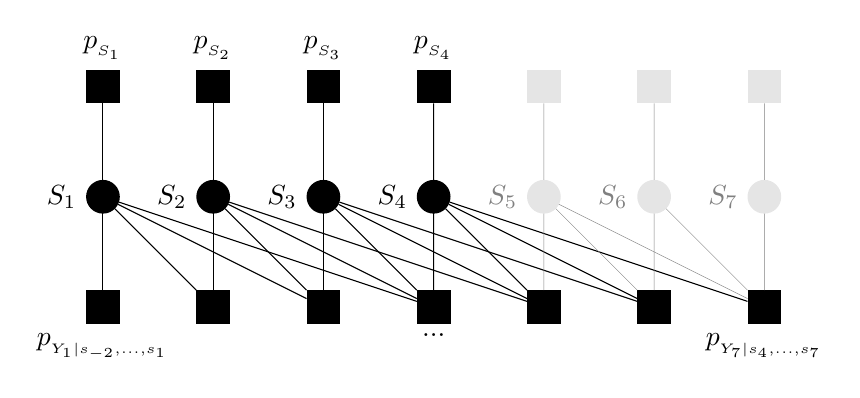
\begin{tikzpicture}[scale=0.7]
\tikzstyle{factor}=[rectangle,minimum size = 4mm, thick, draw =black,fill=black]
\tikzstyle{factorg}=[rectangle,minimum size = 4mm, thick, draw =lgray,fill=lgray]
\tikzstyle{var}=[circle,minimum size = 4mm, thick, draw =black,fill=black]
\tikzstyle{varg}=[circle,minimum size = 4mm, thick, draw =lgray,fill=lgray]
\tikzstyle{connect}=[-latex, thick]


	\node[var] (s0) at (0,2) [label=left:{$S_1$}]{};
	\node[factor] (fs0) at (0,4) [label=above:{$\p{S_1}$}]{};
	\node[factor] (fy0) at (0,0) [label=below:{$\p{Y_1|s_{-2},\ldots,s_1}$}]{};

	\node[var] (s1) at (2,2) [label=left:{$S_2$}]{};
	\node[factor] (fs1) at (2,4) [label=above:{$\p{S_2}$}]{};
	\node[factor] (fy1) at (2,0) [label=below:{}]{};

	\node[var] (s2) at (4,2) [label=left:{$S_3$}]{};
	\node[factor] (fs2) at (4,4) [label=above:{$\p{S_3}$}]{};
	\node[factor] (fy2) at (4,0) [label=below:{}]{};

	\node[var] (s3) at (6,2) [label=left:{$S_4$}]{};
	\node[factor] (fs3) at (6,4) [label=above:{$\p{S_4}$}]{};
	\node[factor] (fy3) at (6,0) [label=below:{$...$}]{};

	\node[varg] (s4) at (8,2) [label=left:{\color{gray}$S_5$}]{};
	\node[factorg] (fs4) at (8,4) [label=above:{}]{};
	\node[factor] (fy4) at (8,0) [label=below:{}]{};

	\node[varg] (s5) at (10,2) [label=left:{\color{gray}$S_6$}]{};
	\node[factorg] (fs5) at (10,4) [label=above:{}]{};
	\node[factor] (fy5) at (10,0) [label=below:{}]{};

	\node[varg] (s6) at (12,2) [label=left:{\color{gray}$S_7$}]{};
	\node[factorg] (fs6) at (12,4) [label=above:{}]{};
	\node[factor] (fy6) at (12,0) [label=below:{$\p{Y_7|s_4,\ldots,s_7}$}]{};

%	\node[var] (s7) at (14,2) [label=left:{$S_7$}]{};
%	\node[factor] (fs7) at (14,4) [label=above:{$\ind[s_7=s^*]$}]{};
%	\node[factor] (fy7) at (14,0) [label=below:{$\p{Y_7|s_4,\ldots,s_7}$}]{};

	
	
	\path
		
		(fs0) edge [] (fy0)
		(fs1) edge [] (fy1)
		(fs2) edge [] (fy2)
		(fs3) edge [] (fy3);

		%(fs7) edge [] (fy7);
                 ;
	\path
		(s0) edge [] (fy1)
		(s0) edge [] (fy2)
		(s0) edge [] (fy3);
	
	\path
		(s1) edge [] (fy2)
		(s1) edge [] (fy3)
		(s1) edge [] (fy4);
	
	\path
		(s2) edge [] (fy3)
		(s2) edge [] (fy4)
		(s2) edge [] (fy5);
	
	\path
		(s3) edge [] (fy4)
		(s3) edge [] (fy5)
		(s3) edge [] (fy6);


	
\path[font=\scriptsize,gray,line width=0.05mm]
		(s6) edge [] (fy6)
		(s5) edge [] (fy6)
		(s5) edge [] (fy5)
		(s4) edge [] (fy5)
		(s4) edge [] (fy6)
		(s4) edge [] (fy4)
		(fs4) edge [] (s4)
		(fs5) edge [] (s5)
		(fs6) edge [] (s6);				

\end{tikzpicture}
%\caption{Factor graph associated to $\p{\S,\ve{\Phi}|\Y=\y}(\s,\ve{\ve{\phi}})$ in \EQ{2.16} }\LABFIG{2.2}
\caption{Factor graph representation of $\p{\S|\y}(\s)$  for the case $\chl=3$ and $\t=4$.}\LABFIG{1.4}
\end{figure}

\begin{exampleblock}{}
This FG has cycles. By clustering nodes we can obtain a cycle-free representation.
\end{exampleblock}


}


\frame{
\begin{itemize}
\item \snoteR{\emph{State} variable at time $k$, $E_k$}. Given a realization of the $\chl$ symbols transmitted immediately before time $k$, i.e., $\sg_{k}=\{s_{k-\chl},s_{k-\chl+1},\ldots,s_{k-2},s_{k-1}\}$, then 
\begin{align*}
e_k=f(\sg_{k}): \AQAM^{\chl} \rightarrow \{1,2,\ldots, M^\chl\}
\end{align*}
\item \snoteG{$E_k$ is a R.V. that takes $M^\chl$ possible values. }
\end{itemize}
\begin{itemize}
\item However, there is a deterministic (one-to-one) relationship between $\sg_{k}$ and $e_k$.
\end{itemize}
}


\frame{
\begin{itemize}
%\item \snoteR{\emph{State} variable at time $k$}. Let $\s_{k}=\{s_{k-\chl},s_{k-\chl+1},\ldots,s_{k-2},s_{k-1}\}$, then
%\begin{align*}
%e_k=f(\s_{k}): \AQAM^{\chl} \rightarrow \{1,2,\ldots, M^\chl\}
%\end{align*}
%\item \snoteG{$e_k$ is a R.V. that takes $M^\chl$ possible values.}
\item The joint posterior probability of the symbols  $\S$ and states $ \seqSt$ can be expressed as 
\begin{align*}
\only<1-4>{\p{\S,\seqSt|\y}(\s,\seqst)=\frac{\snoteR{\p{\Y|\seqst}(\y)}~ \snoteB{\p{\seqSt|\s}(\seqst)}~ \snoteG{\p{\S}(\s)}}{\p{\Y}(\y)}}
\end{align*}
where 
\begin{align*}
\only<1-1>{}
\end{align*}
\begin{align*}
\only<2-4>{\snoteR{\p{\Y|\seqst}(\y)}&=\prod_{k=1}^{\t+\chl}\p{Y_k|\st{k},\st{k+1}}(y_k)}
\\
\only<3-4>{\snoteB{\p{\seqSt|\s}(\seqst)}&=\ind[\st{1}=\st{}^*]\ind[\st{\t+\chl+1}=\st{}^*]\prod_{k=1}^{\t+\chl}
\ind[e_k\cup s_k\rightarrow e_{k+1}]}\\
\only<4-4>{\snoteG{\p{\S}(\s)}&=\prod_{k=1}^{\t+\chl}\p{S_k}(s_k)}
\end{align*}
\end{itemize}



}


\frame{
 If we finally define
\begin{align*}
t_k(\st{k},\st{k+1},s_k)=\p{Y_k|\st{k},\st{k+1}}(y_k)~ \ind[\st{k}\cup s_k\rightarrow \st{k+1}]~ 
\end{align*}
\only<2-2>{
Then...
\begin{exampleblock}{}
\begin{align*}
\p{\S,\seqSt|\y}(\s,\seqst)\propto \ind[\st{1}=\st{}^*] \ind[\st{\t+\chl+1}=\st{}^*] \prod_{k=1}^{\t+\chl} \p{S_k}(s_k)t_k(\st{k},\st{k+1},s_k)
\end{align*}
\end{exampleblock}
}


}

\frame{
\begin{align*}
\p{\S,\seqSt|\y}(\s,\seqst)\propto \ind[\st{1}=\st{}^*] \ind[\st{\t+\chl+1}=\st{}^*] \prod_{k=1}^{\t+\chl} \p{S_k}(s_k)t_k(\st{k},\st{k+1},s_k)
\end{align*}

\begin{figure}[h]
\centering
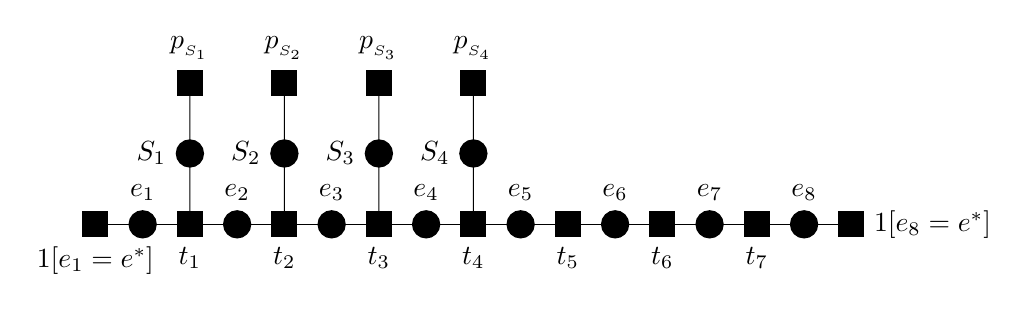
\begin{tikzpicture}[scale=0.3]
\tikzstyle{factor}=[rectangle,minimum size = 3mm, thick, draw =black,fill=black]
\tikzstyle{var}=[circle,minimum size = 3mm, thick, draw =black,fill=black]
\tikzstyle{connect}=[-latex, thick]

	
	\node[factor] (tphi0) at (0,0) [label=below:{$\ind[\st{1}=\st{}^*]$}]{};
	\node[var] (phi0) at (2,0) [label=above:{$\st{1}$}]{};
	\node[factor] (tphi1) at (4,0) [label=below:{$t_1$}]{};
	\node[var] (s0) at (4,3) [label=left:{$S_1$}]{};
	\node[factor] (fs0) at (4,6) [label=above:{$\p{S_1}$}]{};
	
	\node[var] (phi1) at (6,0) [label=above:{$\st{2}$}]{};
	\node[factor] (tphi2) at (8,0) [label=below:{$t_2$}]{};
	\node[var] (s1) at (8,3) [label=left:{$S_2$}]{};
	\node[factor] (fs1) at (8,6) [label=above:{$\p{S_2}$}]{};	

	
	\node[var] (phi2) at (10,0) [label=above:{$\st{3}$}]{};
	\node[factor] (tphi3) at (12,0) [label=below:{$t_3$}]{};
		\node[var] (s2) at (12,3) [label=left:{$S_3$}]{};
	\node[factor] (fs2) at (12,6) [label=above:{$\p{S_3}$}]{};		
	
	\node[var] (phi3) at (14,0) [label=above:{$\st{4}$}]{};
	\node[factor] (tphi4) at (16,0) [label=below:{$t_4$}]{};
	\node[var] (s3) at (16,3) [label=left:{$S_4$}]{};	
	\node[factor] (fs3) at (16,6) [label=above:{$\p{S_4}$}]{};
	
	\node[var] (phi4) at (18,0) [label=above:{$\st{5}$}]{};
	\node[factor] (tphi5) at (20,0) [label=below:{$t_5$}]{};
	%\node[var] (s4) at (20,3) [label=left:{$S_5$}]{};	
	%\node[factor] (fs4) at (20,6) [label=above:{$\p{S_5}$}]{};	
	
	%\node[factor] (fs5) at (24,6) [label=above:{$\p{S_6}$}]{};	
	%\node[var] (s5) at (24,3) [label=left:{$S_6$}]{};	
	\node[var] (phi5) at (22,0) [label=above:{$\st{6}$}]{};
	\node[factor] (tphi6) at (24,0) [label=below:{$t_6$}]{};	
	
	%\node[factor] (fs6) at (28,6) [label=above:{$\p{S_7}$}]{};	
	%\node[var] (s6) at (28,3) [label=left:{$S_7$}]{};	
	\node[var] (phi6) at (26,0) [label=above:{$\st{7}$}]{};
	\node[factor] (tphi7) at (28,0) [label=below:{$t_7$}]{};
	\node[var] (phi7) at (30,0) [label=above:{$\st{8}$}]{};
	\node[factor] (tphi8) at (32,0) [label=right:{$\ind[\st{8}=\st{}^*]$}]{};
	
	\path
		(tphi0) edge [] (tphi8)
		(fs0) edge [] (tphi1)
		(fs1) edge [] (tphi2)
		(fs2) edge [] (tphi3)
		(fs3) edge [] (tphi4);	
				
		
	
\end{tikzpicture}
\caption{Factor graph associated to $\p{\S,\seqSt|\y}$ for the case $\chl=3$ and $\t=4$.}\LABFIG{1.5}
\end{figure}



}

\frame{

\begin{block}{}
Beyond visualization, the fact that the FG in the latter case is cycle-free has important practical implications to construct efficient inference methods. 
\end{block}
\vspace{0.5cm}

Indeed, because of the FG structure the complexity of 
\begin{align*}
\hat{s}_k &=\arg\max_{s_k\in\AQAM} \p{s_k|\y}(\s)=\arg\max_{s_k\in\AQAM} \sum_{\s_{\sim k}\in\AQAM^{\t-1}} \sum_{\seqst} \p{\S,\seqSt|\y}(\s,\seqst)\\
\hat{\s}&=\arg\max_{\s\in\AQAM^\t} \p{\S,\seqSt|\y}(\s,\seqst)
\end{align*}
can be reduced to \noteR{$\mathcal{O}(M^\t)$} to  \noteB{$\mathcal{O}(\t M^\chl)$}.
}


\end{document}

